%!TEX root=../Vorlage_DA.tex
%	########################################################
% 				Travis CI
%	########################################################


%	--------------------------------------------------------
% 	Allgmeine Hinweise
%	--------------------------------------------------------
\newpage
\section{Travis CI}

Travis CI\footnote{\url{https://travis-ci.com}} ist ein System um die kontinuierliche Integration\footnote{\url{https://de.wikipedia.org/wiki/Kontinuierliche_Integration}} von Quellcode zu gew\"ahrleisten. Unter anderem wird \"uberpr\"uft, ob das Projekt \"uberhaupt kompiliert und ob alle Testf\"alle korrekt durchlaufen werden. Wir testen des Weiteren auch das korrekte Starten der Benutzeroberfl\"ache, um grundlegenden Fehler zu vermeiden. Diese sind z.b. vergessene Dateien, welche nicht in das Versionsverwaltungssystem eingecheckt wurden.

Ein besonderer Vorteil von Travis CI ist die einfache Integration in GitHub. Sobald ein Pull-Request oder ein Commit auf dem Server stattfindet, wird dieser getestet. Falls ein Fehler auftritt wird sofort der jeweilige Entwickler informiert, so dass er das Problem schnell beheben kann.

\begin{figure}[h]
\centering
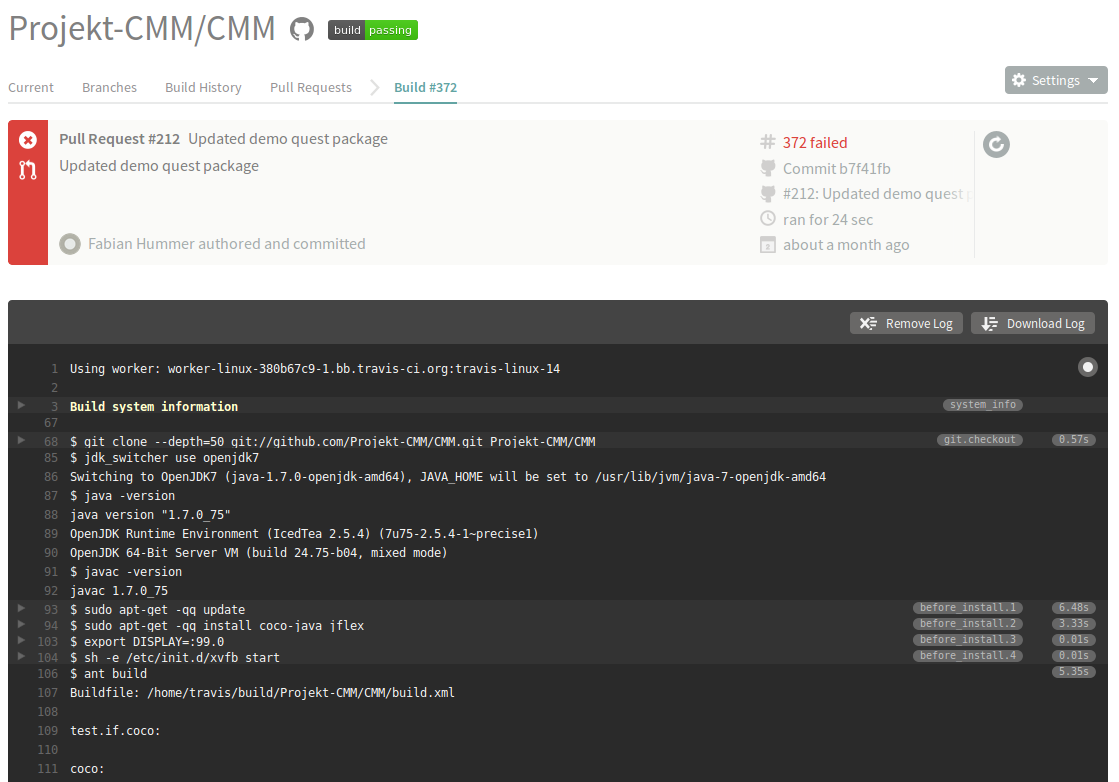
\includegraphics[width=1\textwidth]{./media/images/development/travis_failed.png}
\caption{Fehlgeschlagener Test in Travis CI}
\label{development_travis_failed}
\end{figure}